\chapter{Christmas Yule Log}
\label{ch:yulelog}
\index{dessert}
\index{chocolate}
\index{cake}
\index{Christmas}

Family member: Aunt Joanne

\marginnote[20pt]{\\
    \textbf{Makes 1 yule log} \\
    Prep time: 2-3 hours + setting time in the fridge \\
    Cook time: 15-20 minutes \\
    \vspace*{\baselineskip}

\textbf{Ingredients for the cake:} \\
    5 eggs, separated at room temperature \\
    1 cup confectioners’ sugar \\
    1/8 tsp salt \\
    2 1/2 cups whipping cream \\
    3/4 cup cocoa powder \\
    \vspace*{\baselineskip}

\textbf{Ingredients for the Mocha-Cream Filling:} \\
    3 cups whipping cream \\
    1 cup cocoa powder \\
    1/2 cup confectioners’ sugar \\
    3-4 tbsp Kahlua \\
    \vspace*{\baselineskip}

    \textbf{For decoration (optional):} \\
    Lindt chocolate balls (dark, milk, white) \\
    Raspberries \\
    Chocolate Santa Clause or Snowman \\
}

% \newthought
% \bigskip

\begin{enumerate}
    \item Preheat oven to 400\degree F. Grease the bottom of pan with margarine. Place parchment paper on top, and spray Pam on the parchment paper.
    \item In a large bowl with the mixer at high speed, beat egg whites until soft peaks form. Beating at high speed, gradually sprinkle in 1/2 cup confectioners’ sugar, beating thoroughly after each addition. Continue beating until the egg whites stand in stiff, glossy peaks. Set aside.
    \item In small bowl with same beaters and with the mixer at high speed, beat egg yolks until thick and lemon-colored. Reduce speed to low; beat in the salt, 1/2 cup confectioners’ sugar and 3 tbsp cocoa powder, occasionally scraping bowl with rubber spatula.
    \item Using the wire whisk or rubber spatula, gently fold the yolk mixture into the beaten whites just until the mixture is blended. Spread the batter evenly in the pan and bake 15 minutes or until top springs back when lightly touched with finger.
    \item Prepare a clean cloth towel by sprinkling it with cocoa powder.
    \item When the cake is done, with small spatula, immediately loosen its edges from the side of pan; invert the cake onto the prepared towel. Gently peel the parchment paper from bottom of cake. Roll the towel with the cake from narrow end, jelly-roll fashion. Let it cool completely, placing it seam side down on wire rack.
    \item Meanwhile, prepare the Mocha-Cream Filling. In a large bowl with the mixer at medium speed, beat the whipping cream, cocoa powder, confectioners’ sugar and Kahlua until stiff peaks form.
    \item When the cake is cool, unroll it from the towel and evenly spread the Mocha-Cream Filling on the cake.
    \item Starting at the narrow end, roll up the cake, without the towel this time. Place the cake, seam side down on a platter. Evenly spread the filling on the rolled up cake.
    \item If desired, you can cut a piece at the end of the log cake and place it on the top of the cake – far left side to resemble a knot in the log. Spread the filling on the slice too.
\end{enumerate}

\marginnote{
    You can decorate the top of the log cake either with:
    \vspace*{\baselineskip}
    - Lindt chocolate balls, alternating white, dark, milk chocolate. You can put raspberries between the chocolate balls \\
    - Chocolate Santa Clause or Snowman \\
}

\begin{figure}
  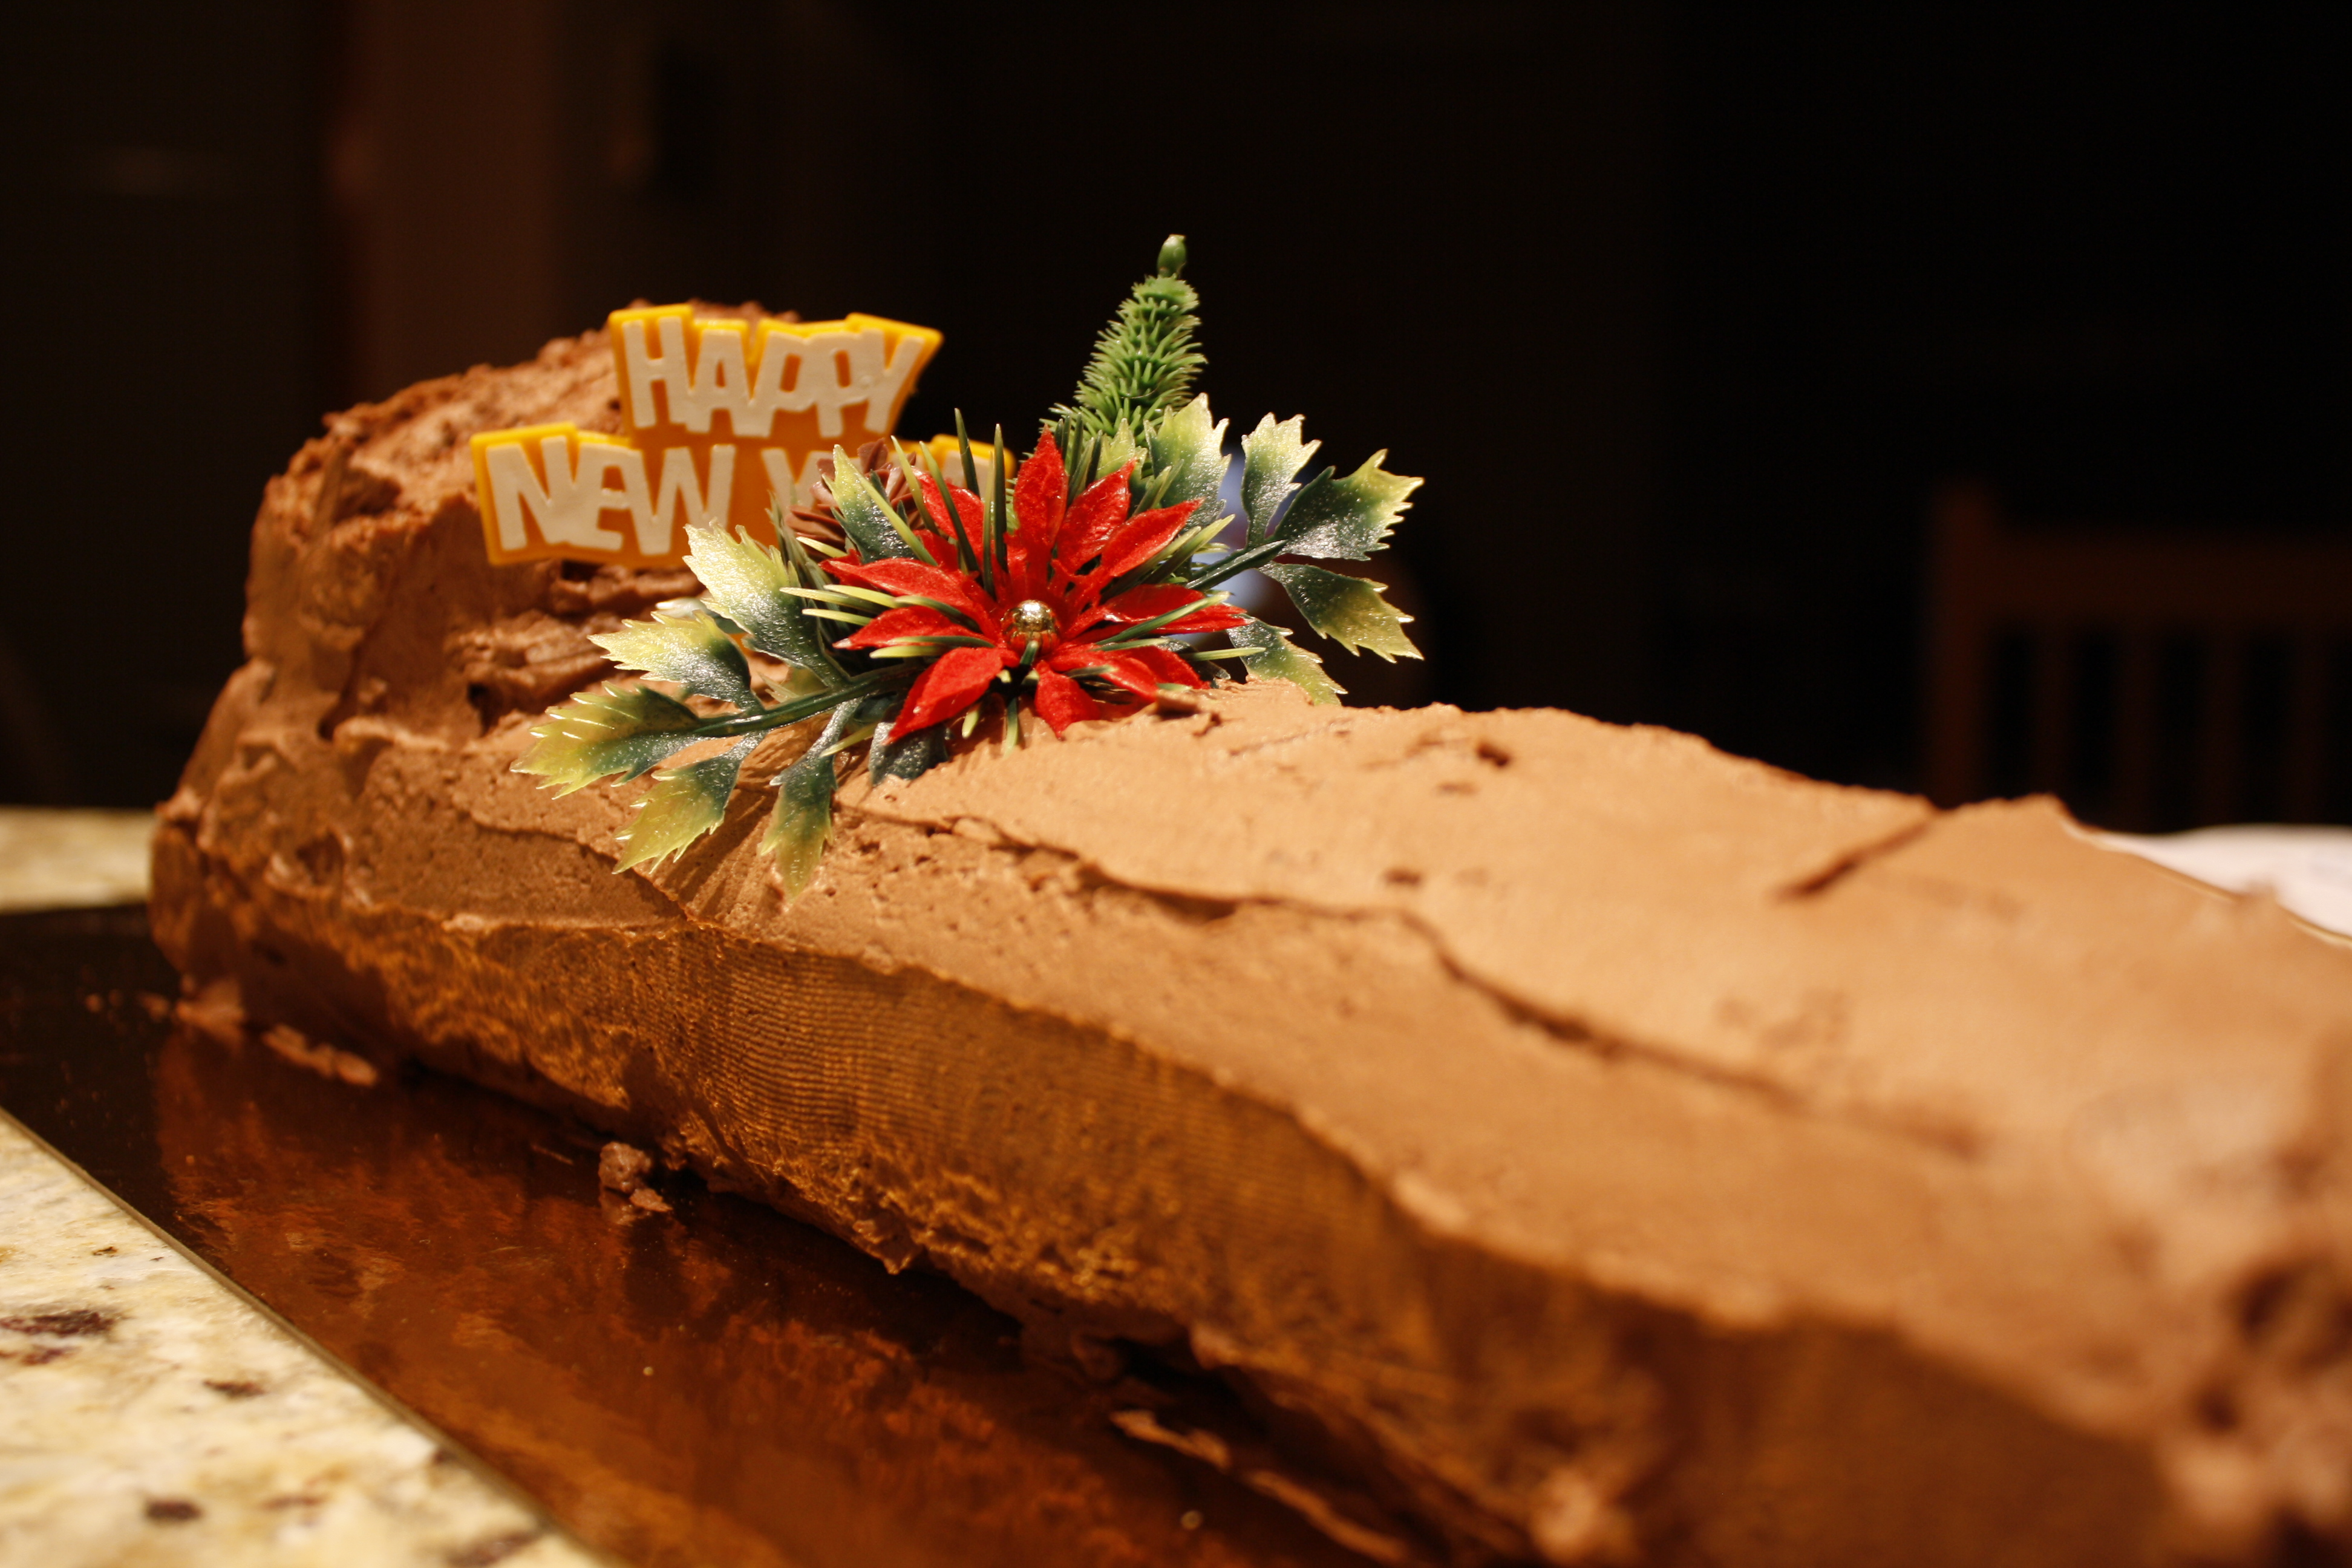
\includegraphics[width=60mm]{dermardiros/images/Logcake.JPG}
    \caption{Yule Log we made with AJ in 2011}
  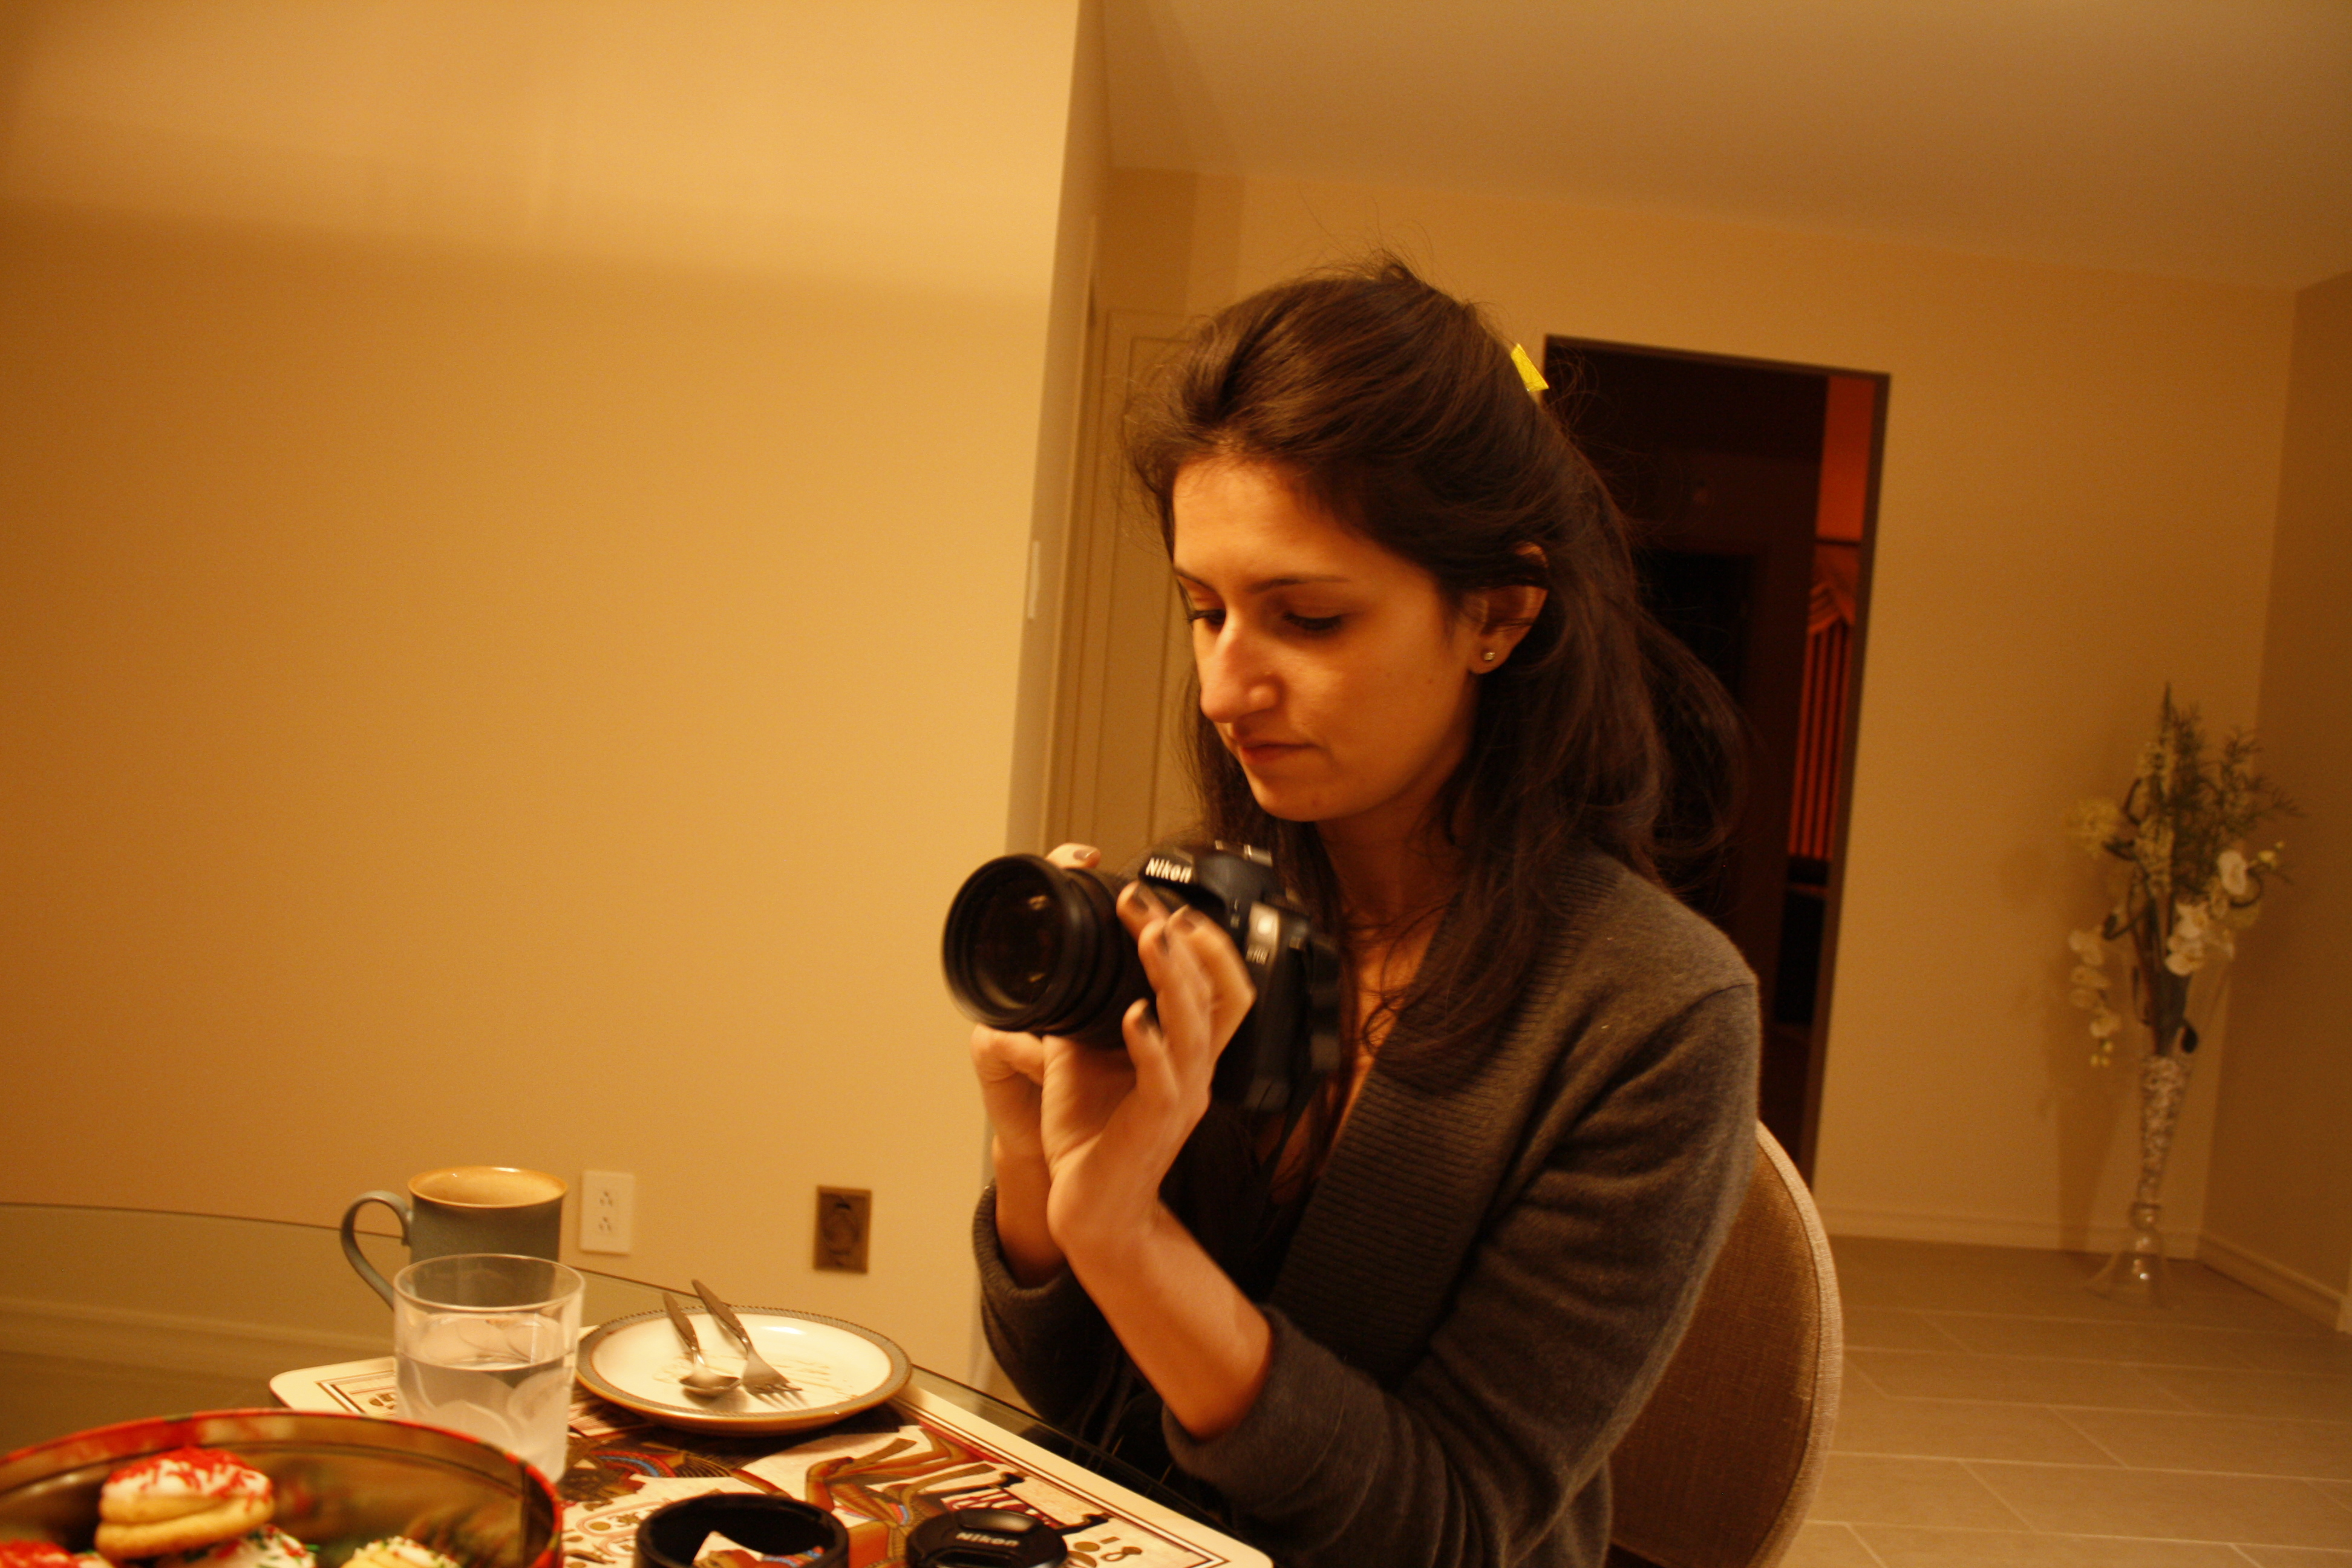
\includegraphics[width=60mm]{dermardiros/images/Logcake 3.JPG}    
\end{figure}